\section{\retro\ Design}

% \begin{figure}[!t]
% \vskip -0.03in
%   \centering
%       {
%         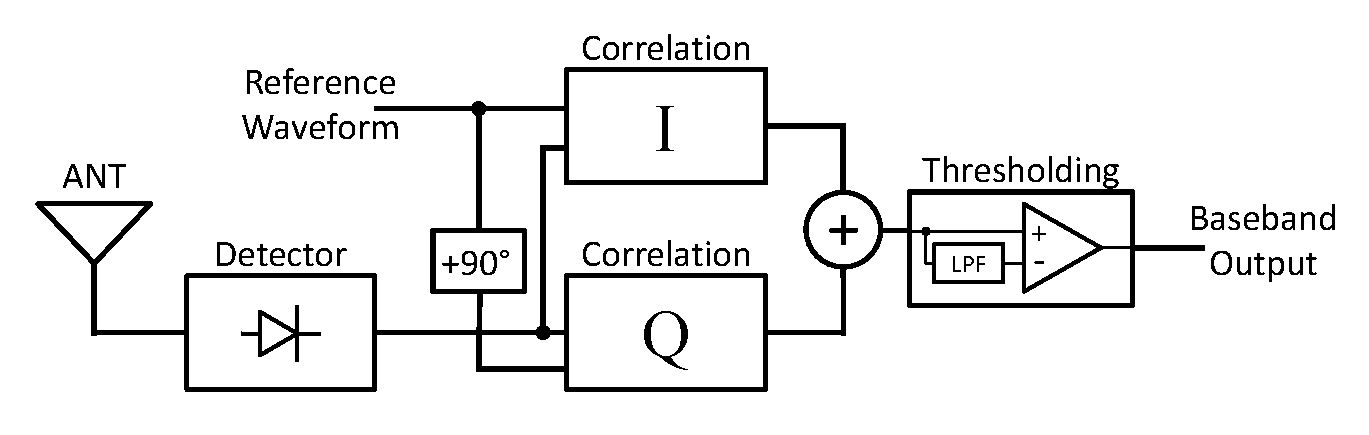
\epsfig{file=../figures/corr-bd.eps, width=0.6\columnwidth}
%       }
% \caption{{\bf System Diagram} (a) \vitag\ and (b) Modified LED.}
% \label{fig:sysdiagram}
% \vskip -0.05in
% \end{figure}

\begin{figure*}[!t]
\vskip -0.1in
\centering
{\footnotesize
\begin{tabular}{cc}
\epsfig{file=../illustrations/tag.eps, width=2\columnwidth} \\ {(a) \vitag\ Block Diagram}\\
\epsfig{file=../illustrations/reader.eps, width=2\columnwidth} \\ {(b) LED Block Diagram}\\
\end{tabular}
}
\vskip -0.1in
\caption{\footnotesize{\bf System Diagram.} Blah Blah.}
\label{fig:sysdiagram}
\vspace{-1em}
\end{figure*}

\retro\ is a new form of communication in which battery-free \vitag\/s can communicate with LEDs without any additional infrastructure. Harvesting LED light energy, a \vitag\ reflects visible light signals to communicate. Because of the ubiquitous deployment of illuminating LEDs, building such a system will enable ubiquitous communications at an unprecedented scale. It will also enhance the security of current RFID systems as it limits the uplink signal exposure to line-of-sight, and the use of retro-reflectors will further focus the signal to an even thiner area, leaving less chance for the hidden attackers and sniffers to temper the system.

Designing such a system, however, faces several challenges, which we will break down in the following subsections, and we describe how our design address these challenges.


%Designing such tags, however, is challenging for four reasons: First, the visible light that carries data is interleaving with intensive interference, such as radios operating at the same frequency, and the light emitted from the LEDs that also carries data and its reflections from surrounding walls, thus making an interference-intensive receiving condition for both \vitag\ and \reader. Second, the signal is exposed to noise, such as the existing environmental lights that is subject to constant changing, human-body-movement-caused noise, and the noise caused by the hardware system itself. Third, to emit modulated light from \vitag\ and make it detectable by \reader\ on a battery-free tag is challenging in that modulating signals on visible light bands is power-consuming with respect to the goal of being battery-free. Finally, to integrate the system to off-the-shelf LED lights while keeping the brightness of the lights constant is challenging. In the rest of this section and the next section, we describe how our design addresses the above challenges.




\subsection{Overview}
Fig.~\ref{fig:sysdiagram} (a) shows a block diagram of our \vitag\ design. It consists of a transmitter, a receiver, an MCU and a harvester. The transmitter and receiver communicate by modulated backscattering of visible light signals, and the harvester absorbs energy from visible lights to power the device. Further, they operate independently of each other. The receiver immediately awakes the MCU by rising the tag voltage to a certain value and enabling the analog circuit to start receiving as it detects a data packet coming in. The MCU then shuts down the analog circuit and powers up the transmitting circuit. The receiving circuit and the transmitting circuit work alternately to save energy. Alongside the communication modules is the energy harvester, which consists of a number of solar cells that transfer visible light energy into electric energy. The harvester sets the upper bound of the power \vitag\ can take on, thus posing a strict constraint to the design of each component on the tag.

Fig.~\ref{fig:sysdiagram} (b) shows a block diagram of our \reader\ design. The major part of it is an LED bulb that emits fast-fluctuating light human eyes cannot detect flickering in. \reader\ builds on off-the-shelf LEDs and makes minor modifications on them. It consists of a transmitter, a receiver and an MCU. The transmitter encodes and modulates the data, feeding the data to the LED for transmission, while keeping the LED not flickering and with dimming support. The transmitter also takes the goal of making \vitag\ battery-free in mind, emitting lights with data such that \vitag\ can demodulate and decode the data at a low energy cost. The receiver deals with the light backscattered from \vitag, and also cancels noise and interference as much as possible. The MCU processes the data transmitted from \vitag.

Next, we describe our design of the transmitter and receiver on the \vitag\ and LED in more detail.





\subsection{\reader\ Transmitter}
\label{subsec:LEDtrans}

As shown in Fig.~\ref{fig:sysdiagram} (b), the transmitter on \reader\ is composed of a crystal oscillator that runs at 1MHz\footnote{The fastest flickering rate of our LED is 1MHz}, and an MCU followed by two amplifiers. The MCU-generated bits toggle the crystal oscillator to OOK the signal with Manchester encoding. The modulated signal will then be amplified and fed to a LED. To make sure the brightness of the LED does not pose a difference between the transmitting and not transmitting state, we add a DC component to the signal. The magnitude of the DC component is adaptable so that we can dim the brightness of the LED emission. In addition to the dimming support, flickers are avoided in \reader\ transmitter. We use 10kHz as the data rate, which far exceeds the frequency (200 Hz) below which human eyes will feel of fluctuations, which could disturbing and unacceptable. 


% We illustrate a typical packet the LED transmits in Fig.~\ref{fig:commdiagram}.

% \begin{figure}[!t]
% \vskip -0.03in
%   \centering
%       {
%         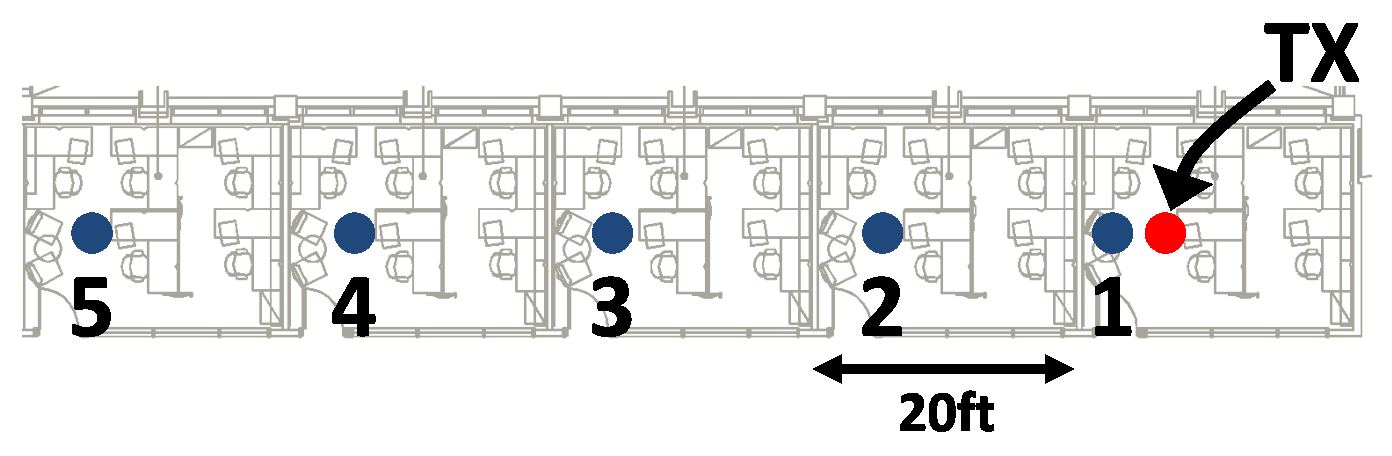
\epsfig{file=../figures/layout2.eps, width=0.6\columnwidth}
%       }
% \caption{{\bf An LED-transmitted Packet} \hl{blah}.}
% \label{fig:commdiagram}
% \vskip -0.05in
% \end{figure}

% We note the following about our design: Firstly, we use a white-colored LED, which emits electromagnetic waves of wavelengths between 380 and 780 nm. The highest flickering frequency of the LED with full on/off transitioning is 1MHz, and we are exploiting the flickering rate to its fullest, in order to leave room for downlink data rate as high as possible. 

% Secondly, different components in the transmitter on the reader side require different voltage supply. We are using two DC/DCs to boost the voltage for the switch and the amplifiers. Specifically, the voltage used for supply the crystal oscillator, the amplifiers for the MCU-output signals and the switch is 5V, and the voltage for the amplifiers for the RF signals is 12V. 

% Finally, the 1MHz frequency, as mentioned earlier, is used because of the full flickering capability we would like to draw from the LED. However, around this frequency with a bandwidth on the order of 100kHz, there are commercial radios using AM modulation. For example, there are radios from 540 through 1610 kHz with 10 kHz spacing in America. Another form is situated at a similar spectrum spanning from 531 to 1611 kHz with 9 kHz spacing. There are also other interferences, which we address in later sections.





\subsection{\vitag\ Receiver}

\begin{tcolorbox}
\vskip 0.05in\noindent{\bf Challenge:} It is power consuming to Demodulate and decode the high throughput LED-transmitted data.
\vskip 0.05in\noindent{\bf Solution Principle:} Use analog components as many as possible (to avoid ADCs) and avoid complicated digital signal processing on the mobile end. Also, design amplifiers that work at an almost-cut-off state to save energy cost.
\end{tcolorbox}

Following the flow of the signal, we describe the design of our \vitag\ receiver. We first use a light sensor\footnote{A normal light sensor has a bandwidth of over 1GHz} that captures the visible light. The captured signals then go through filters, detectors/demodulators, and another feedback amplifier before being sent to a comparator be digitized. We only use analog elements and a low-power microcontroller for receiving, and design modules that set the amplifiers to work at an almost-cut-off state, where the energy consumption is extremely low. The block diagram of the receiver is presented in Fig.~\ref{fig:sysdiagram} (a).

\subsubsection{Extracting Information from the Visible Light}
\reader\ transmitted signals are captured with a light sensor. The light sensor has an equivalent capacitance, which, with an inductor parallel to it, performs preliminary front-end filtering. Next, two amplifiers successively amplify the RF signal while avoiding auto-excitation using a feedback mechanism. Upon preliminary filtering and amplification, the signal is ready for demodulation. Avoiding the downside of a conventional envelope detector on high power consumption, our demodulator contains a constant current source, a diode, and a frequency selection amplifier. The constant current source sets the current that flows into the base of the triode in the frequency selection amplifier, making it work at an almost-cut-off state, such that the amplifier is turned on and the signal is amplified when the positive half of the signal that has an average of 0 flows in. On the other hand, when the negative half of the signal flows in, the amplifier is turned off. This process essentially demodulates the signal from the 1MHz carrier. Finally, the signal passes through an RC filter, which further smooths the signal, ready to be fed to a comparator for digitization. Overall, our demodulator saves more energy than a conventional envelope detector because of the low-energy working region ours works in. We also note that the output of our demodulator is smoother, while having a higher gain than a traditional envelope detector, which is favorable in the energy-constrained decoding phase.

\subsubsection{Decoding on an Ultra-Low-Power Device}

While the output of the envelope detector is a smooth wave, it is still analog with continuous values. In principle, a receiver with an ADC can distinguish between the two signal levels by processing the digital samples. Specifically, say we have two signals with different voltages, $V_0$ and $V_1$, $V_0 > V_1$, where $V_0$ and $V_1$ correspond to the power levels for the zero and one bits. To distinguish between them, the receiver would first compute a threshold value. If the duty cycle of the signal is $50\%$, and odds of the occurrence of zeros and ones are equal, then the threshold is the average of the two power levels. If the received signal is greater than this threshold, we conclude that the received signal is $V_1$; else, we conclude that the received signal is $V_0$.

Since we seek to eliminate the need for a full ADC in order to reduce power, the receiver should imitate this operation using analog hardware. In favor of Manchester coding we use (see~\ref{subsec:LEDtrans}), the goal of our design, however, is different from a typical ADC. The Manchester-encoded signal uses edges to denote bits. Specifically, an up edge denotes one, and a down edge denotes zero. To align with this pattern, we design a comparator that detects changes of the voltage. First, using a resister and a capacitor, the comparator sets a time constant that features its detection delay that corresponds to the input data rate. The comparator consistently compares the current analog value $V_{now}$ with the signal value at the last bit $V_{previous}$. If $V_{now} > V_{previous}$, the comparator outputs $1$; otherwise, it outputs $0$. We note that while a traditional design only performs absolute comparison, our design traces the relative changes in the voltage. Further, using a traditional detector would lead to jagged waveform, which would further cause false comparison results at any edge-based comparator. Instead, our comparator design is more suitable for Manchester coding, which is widely adopted for preventing long consecutive $1$s or $0$s in a bit stream, in avoidance of picking a threshold value that would suffer from drifting. 

THe microcontroller then works to check the correctness of the packet. In the receiving phase, microcontroller consumes $120\mu A$.





\subsection{\vitag\ Transmitter}
\label{subsec:tagtrans}

\begin{tcolorbox}
\vskip 0.05in\noindent{\bf Challenge:} Transmitting with the LCD at a high toggling frequency consumes even more power than the receiver.
\vskip 0.05in\noindent{\bf Solution Principle:} Recycle energy spared by the LCD at every toggle; And use an RC oscillator instead of the crystal oscillator used in the receiving phase.
\end{tcolorbox}


Our \vitag\ transmitter transmits by passively backscattering the incoming light. The core of the transmitter is the combination of an LCD and a retro-reflector that serves as a modulator. To conserve energy, we design an energy reuse module that, in every modulation cycle, recollects $50\%$ of the energy that would have been wasted by the LCD without such a module. To further save energy, instead of using power-demanding crystal oscillators, we use a simple RC oscillator to generate control signals to toggle the LCD. While the RC oscillator does have worse clock stability and a lower frequency, we design modules that address these issues in~\ref{subsec:LEDreceiver}. Finally, the LCD requires a voltage high enough to drive it to its fullest capacity, and this high voltage cannot be directly fed by the low voltage the solar cell can provide. We design a voltage boosting module that achieves this. The overall design of the \vitag\ transmitter is presented in Fig.~\ref{fig:sysdiagram} (a). We now break down the design into the following key points.

\subsubsection{Modulating the Retro-Reflector with an LCD}
To avoid actively generating light signals, which may cost way more power than affordable on a battery-free \vitag, we instead take the advantage of retro-reflectors that passively bounce the incoming light back. As described in Section~\ref{sec:background}, the retro-reflector has the merit that it can directionally bounce the light at a direction same as the one the light arrives at. To modulate the light, we cover the retro-reflector with an LCD. When at work, as electromagnetic waves hit the LCD, the LCD lets the light pass through or blocks it depending on the polarization, i.e., the orientation of the liquid-crystal molecules, in the LCD, which is controlled by the voltage added on it. If the applied voltage is large enough, the pixels will appear black. The highest voltage applied to our LCD that turns it completely black is $6.1V$, and the lowest voltage with which it starts to be polarized is $2.1V$. We are able to flicker it as fast as $1kHz$, which also is our highest data rate on the uplink. Note, that there are other voltage-controlled reflective materials existing that may have higher flicking rate or lower power. Applying one of those in the system might enhance the energy efficiency and the capacity of the system.  

\subsubsection{Energy Reuse}
The current that feeds the LCD which has an equivalent capacitance of $9nF$ would be wasted to the ground when the LCD discharges. However, we found that by recollecting this portion of the current in the LCD discharging phase, $50\%$ of the energy could be saved. In response, we designed an energy reuse module, illustrated in Fig.~\ref{fig:energyreuse}, that features a DC/DC converter that boosts the voltage from the lowest voltage that triggers the LCD to the highest. The lowest voltage, as mentioned earlier, is $2.1V$, which is about the voltage the solar cell array can supply. 

In the charging phase, in which the LCD turns to the blocking mode, the DC/DC boosts the voltage the solar cell supplies to one the LCD reaches its full capacity at. This voltage effectively applies to the LCD when the MCU sets $T_0$ to open, while $T_1$ is set to close. The voltage on the LCD pumps up to $6.1V$ and stays until the discharging phase.

In the discharging phase, the MCU sets $T_0$ to close, and $T_1$ to open. Since there is a diode that blocks the only path along which the LCD could discharge towards the ground, the current that flows from the discharging LCD does not go straight to the ground; Instead, it flows back to the DC/DC, charging $C_0$ and $C_1$, until the voltage on the LCD equals to that on the solar cell. 

We note two things about our design. First, the two signals that control the on/off state of the switches are generated by an MCU. When one of the two is set to high, the other is set to low, and vice versa, As a result, there is only one triode between $T_0$ and $T_1$ open at a time, so the LCD is either in a charging phase or in a discharging phase, with no conflict. Second, we always make sure that the data rate is slower than the rate at which the two signals from the MCU alternate, so that the LCD alternates in a balanced manner without saturation in a long run, i.e., $C_0$ and $C_1$ will not constantly be charged or discharged. In real world settings, fortunately, the \vitag\ has up to $1kbps$ data rate, which is much smaller than the average time used for charging an empty LCD or discharging a full LCD.

\begin{figure}[!t]
\vskip -0.03in
  \centering
      {
        \epsfig{file=../illustrations/EnergyReuseCircuits.eps, width=0.6\columnwidth}
      }
\caption{{\bf Our Energy Reuse Module} \hl{blah}.}
\label{fig:energyreuse}
\vskip -0.05in
\end{figure}





\subsection{\reader\ Receiver}
\label{subsec:LEDreceiver}

\begin{tcolorbox}
\vskip 0.05in\noindent{\bf Challenge:} The LED receiver must handle time offsets caused by the \vitag's RC-based clock with low oscillating frequency, and has to detect the retro-reflected signal which is 3 orders of magnitude weaker than interfering LED transmissions.   
\vskip 0.05in\noindent{\bf Solution Principle:} Design a sliding-window multi-symbol match filter algorithm to remedy clock drifts and LCD-caused signal distortions.
\end{tcolorbox}

The \reader\ captures the signal transmitted by \vitag\ at an up to $1kbs$ data rate on a 1MHz carrier. Upon transferring the light signal to voltage, the \reader\ receiver demodulates and decodes the data using RF-end analog circuits and the same microcontroller the \reader\ transmitter uses. While there is less power limit on \reader\ than \vitag, the \reader\ receiver design still faces multi-fold challenges. (1) First, the signal sent by the \vitag\ is mixed with the \reader-transmitted signal, which, too, is on a 1MHz carrier. Since the \reader\ receiver is much closer to the \reader\ transmitter than the \vitag\ transmitter, the strength of the \reader-transmitted signal with the reflections of this signal by the surroundings 3 orders of magnitude greater than the \vitag-transmitted signal on \reader. As we measure, the typical voltage of the received signal is on the order of magnitude of $mV$, while the voltage supply for the LED receiver is $8V$. (2) Second, the signal carried on 1MHz to be sent by the \reader\ transmitter can also leak to the light sensor, which exacerbates the interference. (3) Third, commercial radios that run on 1MHz could also interfere with the signal that carries useful information. (4) Fourth, the noise caused by the movement of humans and other objects around could be huge. The voltage output of the light sensor on the \reader\ is therefore prone to saturating. (5) On top of these, as we noted in~\ref{subsec:tagtrans}, the received signal suffers from timing offsets caused by the low-cost low-frequency clock on the \vitag. In the rest of this section, we describe our \reader\ receiver design (Fig.~\ref{fig:sysdiagram} (b)) that addresses these challenges.

\subsubsection{Extracting Backscatter Information from noise}
Since the signal to interference ratio is extremely low (~mV against ~V), we have to amplify the received signal more than $1000$ times in magnitude. Using a single amplifier though, is not feasible, as the potential of introducing self-excitation to the circuit with a huge amplification is high, and the noise introduced by a single amplifier tends to be unacceptable. So we apply five successive amplifiers instead. The detailed design is the following. To extract the useful information from the noisy background, we first apply an amplifier at the RF end. This amplifier directly follows the light sensor with an LC filter that performs preliminary band-pass filtering. Subsequently, we add a differential amplifier following a transmission line which decouples the transmitted signal from leaking towards the RF end. There is an impedance matching module between the light sensor filter and the transmission line. Now, the center frequency of the differential amplifier is $1MHz$ with the help of an LC module, and its gain is controlled by the microcontroller. The third and fourth amplifiers are also with LC modules that perform further RF-band filtering. The fourth amplifier is with feedback mechanism. The use of this amplifier is to further increase the signal gain and filter the residual RF-band noise, while dragging the circuit state farther from self-excitation. After the amplifications, this signal is sent to an envelope detector, which performs regular demodulation that picks out the baseband signal from the $1MHz$ carrier. Finally, the same comparator used on the \vitag\ is used to digitize the Manchester-encoded signal.  


\subsubsection{Decoding in the Presence of Clock Offsets}
\label{subsubsec:clockoffset}

Traditionally, the following approaches have been used to extract the timing information from the signal and perform the decoding thereafter.

\vskip 0.05in\noindent{\bf Peak (edge) detection-based algorithms} are ones where samples are taken differentials, and so the extreme (discontinuous) points in the signal are found which denote the clock beats. However, as shown in Fig.~\ref{fig:dynamicRange}, the signal received has a huge dynamic range. If the signal appears to be the case in (a), (b) or (c), the peak approach will fail, as the peak detected will always be ahead of or behind the actual one. In other cases, the edge approach will fail, as the edge is not clearly identified. 
\vskip 0.05in\noindent{\bf Averaging-based algorithms} are ones where samples of the signal are averaged to generate a threshold, and samples above this threshold denote ones and below denote zeros. However, as shown in Fig.~\ref{fig:dynamicRange} (e), when the average value of the signal within a packet is drifting, which may happen for the reasons explained earlier, this approach will likely fail. While one could identify a trend for the change in the average value, it is hard to accurately do so in practice. The reason for this is that as the average value is changing in a coherent way, a wrong prediction of the average value will cause severe errors in the process of decoding.
\vskip 0.05in\noindent{\bf Multi-symbol correlation algorithms} use a string of symbols to represent one bit, and does correlation on the receiver side to decode the bit by finding the peak of the correlation result. The algorithm can pinpoint the clock and hence decode the signal in a low SNR situation, but it is not suitable for low symbol-rate channels like the uplink in our case. 
\vskip 0.05in\noindent{\bf One-symbol match filter algorithms} try to match the wave form of the signal and detects the convolution peaks to determine the accurate timing. However, due to the rough equivalence of the LCD on the tag side that shapes a bit and a capacitor, the basic wave form tends to be sawtooth, as shown in Fig.~\ref{fig:dynamicRange} (d) when there is no top or bottom truncation. Further, as the bits are encoded in Manchester code, the rising edge and the falling edge are not necessarily symmetric in time. A typical example is three chips that contain one high-volt chip followed by two low-volt chips, in which case the correlation peak will be skewed, compared to the case where the voltage is high for one chip and low for the next. Therefore, the timing will be biased.

We develop a novel algorithm to decode the signal encoded with Manchester code that has a large dynamic range. We term it a sliding-window multi-symbol match filter algorithm. The approach extends the one-symbol match filter to that with an addition regarding clock adjustment using a multi-symbol match filter. The basic idea is to avoid the biased timing caused by skewed correlation peaks that happen in the one-symbol match filter case, by matching all possible patterns of the wave form the Manchester-encoded signal appears to have, and iteratively adjusting the local clock by every bit period. To begin with, the algorithm exploits standard correlation to detect the preamble of a packet, using the fact that the preamble is different from any possible bit patterns in the payload. Upon finding the start of a packet, the algorithm estimates the length of a bit first using the knowledge of the \vitag\ clock that has a known frequency yet subject to offsets. Then the algorithm iteratively does the following two things:

\vskip 0.05in\noindent{\bf Step 1: Wave Form Recognition.} As every bit is Manchester-encoded, one bit contains two chips. A bit-period of a square wave that contains a high volt chip and a low volt chip (not necessarily in this order) correlates against the first three bit-periods of the signal. After this, the algorithm knows what these three bits are out of eight possible wave forms.

\vskip 0.05in\noindent{\bf Step 2: Local Time Recovery.} Then the algorithm adjusts the clock estimation by correlating the three bits from the raw signal against the corresponding gold pattern from the eight patterns. Ideally, the correlation yields a peak in the middle of the three bits. However, due to the time variance with the start of the packet and the frequency deviation between the reader clock and the tag clock, the peak of the correlation result does not necessarily align with the ideal peak. To bound the clock estimation error along the bits in a packet, we perform linear regression $t=k\dot s+s_0$ to estimate the timing of the next three bits, using the estimate of the beginning of the packet as $s_0$ and the estimate of the current three bits and their timing as the training data ${s,t}$. Every round $k$ is re-estimated, and then the algorithm moves the three-bit window one bit forward, and jumps back to perform step one, until reaching the end of the packet. This time recovery algorithm designed specifically for our coding and modulation bounds the error on $k$ from propagating as the decoding proceeds. We formally describe this in the following lemma, for which we give a proof in Appendix.


\begin{lemma}
The time recovery renders the clock estimation error's convergence to zero if a packet contains infinite number of bits. 
\label{lem:lemma1}
\end{lemma}


We note that we choose a three-bit time span as a correlation unit because three bits are the smallest number of bits that contain all possible wave forms when the signal is Manchester-encoded and LCD capacitor-filtered.

Following the local time recovery and decoding, \reader\ checks the correctness of the bits received using CRC8. The polynomial used is $x^8 + x^2 + x + 1$.


% \begin{figure}[!t]
% \vskip -0.03in
%   \centering
%       {
%         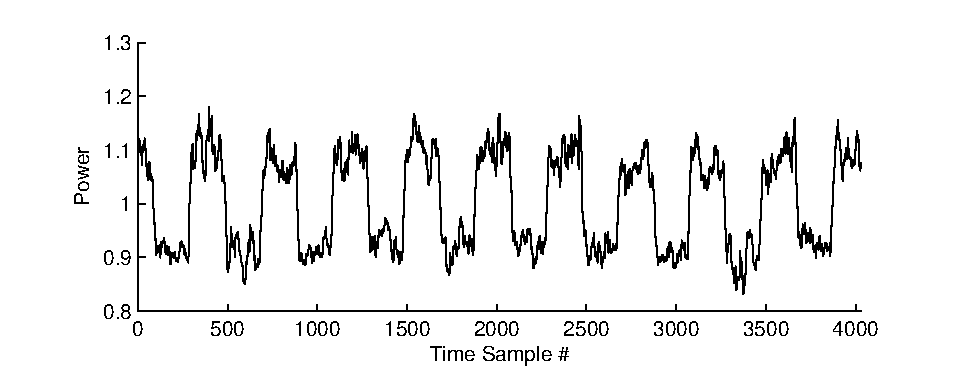
\epsfig{file=../figures/divide.eps, width=0.6\columnwidth}
%       }
% \caption{{\bf Signal Captured by the LED Light Sensor \hl{replace with a system block diagram!!}} \hl{integrates both mmm in a single design. It can operate using both RFID and TV transmissions}.}
% \label{fig:capture}
% \vskip -0.05in
% \end{figure}





\begin{figure*}[!t]
\vskip -0.1in
\centering
{\footnotesize
\begin{tabular}{ccccc}
\epsfig{file=../illustrations/waveform1.eps, width=0.35\columnwidth} & \epsfig{file=../illustrations/waveform2.eps, width=0.35\columnwidth} & \epsfig{file=../illustrations/waveform3.eps, width=0.35\columnwidth} & \epsfig{file=../illustrations/waveform4.eps, width=0.35\columnwidth} & \epsfig{file=../illustrations/waveform5.eps, width=0.35\columnwidth}\\
{(a) Normal} & {(b) Up-truncated} & {(c) Down-truncated} & {(d) Up and Down-truncated} & {(e) Average-drifted}\\
\end{tabular}
}
\vskip -0.1in
\caption{\footnotesize{\bf Varying Wave patterns.} Blah Blah.}
\label{fig:dynamicRange}
\vspace{-1em}
\end{figure*}